\chapter{Simulation Setup and Methodology}

This chapter details the simulation methodology adopted to evaluate the performance of a rectangular microstrip patch antenna (MSPA) under different conditions—specifically, in free space and enclosed within a flat radome. The antenna was designed for 6~GHz operation using an FR4 substrate, modeled and simulated using ANSYS HFSS. The methodology draws from standard antenna theory \cite{balanis} and radome design guidelines provided in \cite{swra705}.

\section{Design Specifications and Calculated Parameters}

The fundamental design inputs for the patch antenna are presented in Table~\ref{tab:designspecs}. These were used to calculate the required dimensions and parameters using standard MSPA design equations.

\begin{table}[htbp]
\centering
\caption{Patch Antenna Design Specifications}
\begin{tabular}{lc}
\toprule
\textbf{Parameter} & \textbf{Value} \\
\midrule
Operating frequency ($f_r$) & 6 GHz \\
Dielectric material & FR4 \\
Relative permittivity ($\varepsilon_r$) & 4.4 \\
Substrate thickness ($h$) & 1.6 mm \\
Loss tangent ($\tan \delta$) & 0.02 \\
\bottomrule
\end{tabular}
\label{tab:designspecs}
\end{table}

Using standard patch antenna equations, the calculated parameters are shown in Table~\ref{tab:calculatedvalues}:

\begin{table}[htbp]
\centering
\caption{Calculated Patch Antenna Parameters}
\begin{tabular}{lc}
\toprule
\textbf{Parameter} & \textbf{Value} \\
\midrule
Patch width ($W$) & 15.126 mm \\
Patch length ($L$) & 11.320 mm \\
Inset feed distance & 3.614 mm \\
Feed line width & 2.990 mm \\
Inset width & 4.600 mm \\
Inset depth & 3.800 mm \\
Effective permittivity ($\varepsilon_{\text{eff}}$) & 3.830 \\
Effective length ($L_{\text{eff}}$) & 12.774 mm \\
Fringing length ($\Delta L$) & 0.723 mm \\
Edge impedance & 284.13 $\Omega$ \\
\bottomrule
\end{tabular}
\label{tab:calculatedvalues}
\end{table}

\section{HFSS Simulation Workflow}

The antenna was modeled in ANSYS HFSS based on the above specifications using the following simulation steps:

\begin{itemize}
    \item Creation of the patch, ground plane, feed line, and substrate geometry.
    \item Assignment of FR4 as the substrate material with appropriate dielectric and loss properties.
    \item Application of waveports to excite the antenna.
    \item Radiation boundary setup to mimic free-space conditions.
    \item Mesh refinement using adaptive meshing for improved solution accuracy.
    \item Solution sweep over frequency range to obtain $S_{11}$ and gain plots.
\end{itemize}

\section{Flat Radome Design and Placement}

A flat radome was introduced to study its influence on antenna characteristics. The radome was modeled as a planar dielectric cover and designed using optimal thickness expressions provided in \cite{swra705}:

\begin{equation}
t_{\text{optimum}} = n \cdot \frac{\lambda_0}{2 \sqrt{\varepsilon_r}},
\end{equation}

where:
\begin{itemize}
    \item $n$ is a positive integer,
    \item $\lambda_0$ is the free-space wavelength,
    \item $\varepsilon_r$ is the radome material's relative permittivity.
\end{itemize}

The radome was placed at a specific spacing from the antenna to minimize reflections and multipath effects. This optimal separation is given by:

\begin{equation}
D_{\text{opt}} = n \cdot \frac{\lambda_0}{2}
\end{equation}

\begin{figure}[H]
\centering
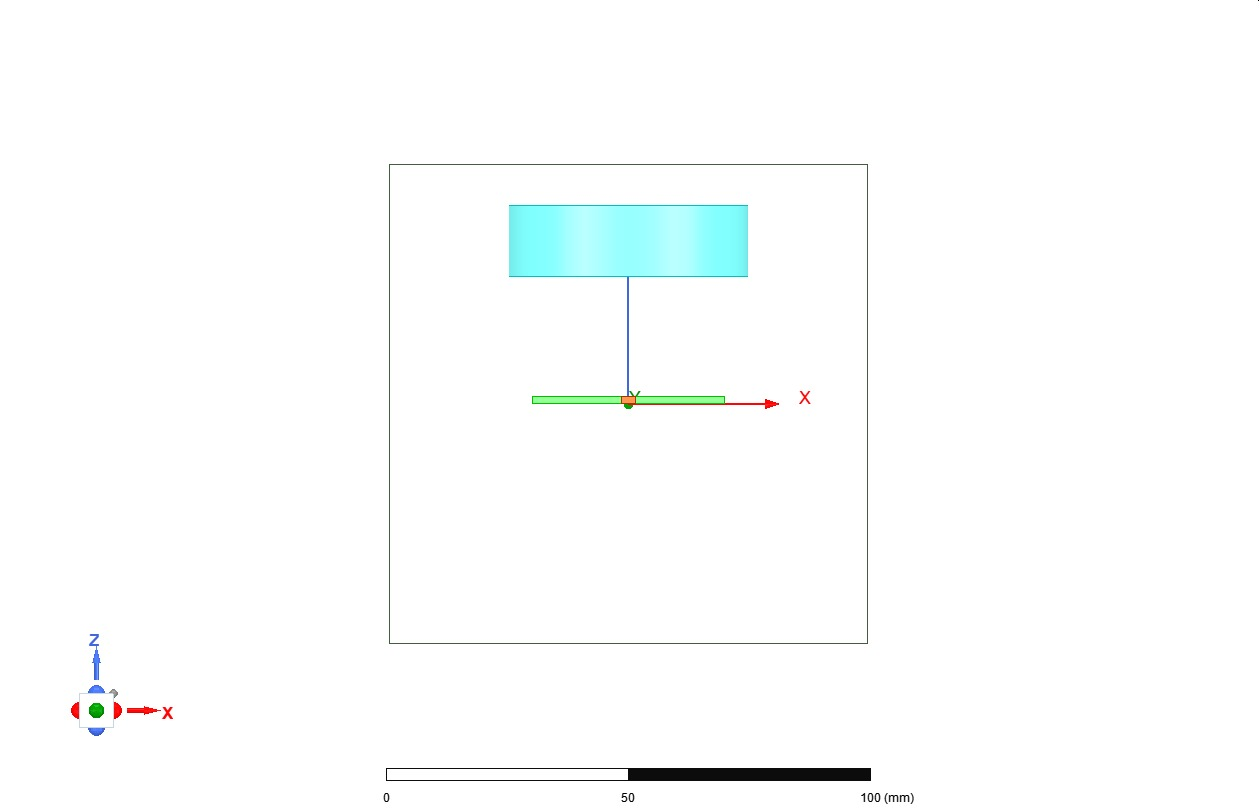
\includegraphics[width=0.8\textwidth]{figures/flat_radome.jpeg}
\caption{Front view of the simulation setup showing the patch antenna enclosed within a flat PMMA radome in ANSYS HFSS.}
\label{fig:flat_radome}
\end{figure}

\subsection*{Radome Material Selection}

In this study, the flat radome was modeled using PMMA (Plexiglass), which is commonly used for RF enclosures due to its mechanical strength and RF transparency. The material parameters used in ANSYS HFSS are listed in Table~\ref{tab:pmma-properties}.

\begin{table}[H]
\centering
\caption{Material Properties of PMMA Used in Simulation}
\begin{tabular}{lcl}
\toprule
\textbf{Parameter} & \textbf{Value} & \textbf{Units} \\
\midrule
Relative permittivity ($\varepsilon_r$) & 2.8 & -- \\
Relative permeability ($\mu_r$) & 1 & -- \\
Dielectric loss tangent ($\tan\delta$) & 0.001 & -- \\
Bulk conductivity & $1 \times 10^{-16}$ & S/m \\
Mass density & 1180 & kg/m$^3$ \\
Measured frequency & 6 GHz & Hz \\
\bottomrule
\end{tabular}
\label{tab:pmma-properties}
\end{table}

\section{Simulation Campaign}

The following simulation cases were conducted in ANSYS HFSS:

\begin{enumerate}
    \item Patch antenna in free space (baseline)
    \item Patch antenna enclosed by a flat PMMA radome
\end{enumerate}

In each case, key performance metrics were extracted, including return loss ($S_{11}$), VSWR, gain patterns, and 3D radiation plots. These results are analyzed and compared in the following chapter.

\section{Outlook for Future Work}

While this study primarily focused on evaluating the influence of flat radomes, several future directions can enhance the simulation methodology:

\begin{itemize}
    \item \textbf{Design Optimization:} Use of metaheuristic algorithms (e.g., genetic algorithms, PSO) to optimize patch dimensions and radome thickness.
    \item \textbf{Advanced Substrates:} Exploration of low-loss substrates like Rogers RT/duroid series for high-performance designs.
    \item \textbf{Environmental Effects:} Study of temperature and humidity influence on dielectric properties and antenna performance.
    \item \textbf{Multi-layer Radomes:} Evaluation of layered dielectric structures for enhanced frequency selectivity and mechanical robustness.
\end{itemize}

These extensions would strengthen the practical applicability of the proposed antenna system, particularly for radio astronomy or high-frequency communication applications.

\section*{Conclusion}

This chapter described the complete simulation pipeline—from calculating patch dimensions to radome modeling in HFSS. The flat PMMA radome was modeled using realistic material parameters, and the simulation configurations were designed to compare the antenna’s free-space performance with radome-enclosed behavior. In the next chapter, we present and interpret the results of these simulations, analyzing key metrics like return loss, gain, and radiation pattern.
